\documentclass[12pt,a4paper,oneside]{book}
\usepackage[utf8]{vietnam}
\usepackage{amsmath, amsfonts, amssymb, graphicx, mathrsfs}
\usepackage{enumerate, boxedminipage, multicol, etoolbox}
\usepackage[shortlabels]{enumitem}
\usepackage{setspace}

%Gói căn lề giấy.
\usepackage[top=2cm, bottom=2cm, left=1.5cm, right=1.5cm]{geometry}

%Xoá thụt đầu dòng.
\setlength\parindent{0pt}

%Gói màu sắc.
\usepackage[dvipsnames]{xcolor}

%Định nghĩa màu.
\definecolor{mauChuDao}{HTML}{1B3D9F}
\definecolor{cqcqcq}{rgb}{0.7529411764705882,0.7529411764705882,0.7529411764705882}
\definecolor{ocre}{RGB}{24,190,250}
\definecolor{ffqqqq}{rgb}{1.,0.,0.}
\definecolor{qqqqff}{rgb}{0.,0.,1.}
\definecolor{ffffff}{rgb}{1.,1.,1.}
%Gói Tikz.
\usepackage{tikz, tkz-tab, tkz-euclide}
\usetikzlibrary{calc, patterns, shadings, angles, intersections, shapes, quotes, trees}

%Gói ex_test.
%\usepackage[dethi]{ex_test}
\usepackage[loigiai]{ex_test}
%\usepackage[book]{ex_test}
\renewcommand{\loigiaiEX}{\centerline{\color{mauChuDao}\faKey~Hướng dẫn giải}}

%Tạo các môi trường mới.
\usepackage[skins,breakable]{tcolorbox}
\usepackage[explicit,calcwidth]{titlesec}
\usepackage{titletoc}
\usepackage{varwidth}
\tcbuselibrary{raster}
\setcounter{secnumdepth}{4}
\setcounter{tocdepth}{1}

%========= Công thức toán =========%
\everymath{\displaystyle}
%Dấu hệ hoặc.
\newcommand{\hoac}[1]
{
	\left[\begin{aligned}#1\end{aligned}\right.
}
%Dấu hệ và.
\newcommand{\heva}[1]
{
	\left\{\begin{aligned}#1\end{aligned}\right.
}
%==================================%

%=======Tùy biến môi trường =======%
\makeatletter
%Tùy chỉnh Mục lục
\usepackage{ifoddpage}
\titleformat{name=\chapter,numberless}[display]
{\normalfont\huge\bfseries}
{}
{-1cm}
{%
	\begin{tikzpicture}[remember picture, overlay]%
		\draw[fill=blue,draw=blue, rounded corners=15pt] (12.5,-.75) rectangle (20,1.3);%
		\draw (13.5,0.2) node [right]{\color{white}\fontsize{25pt}{1pt}\fontfamily{qag}\selectfont\bfseries\MakeUppercase{#1}};%
	\end{tikzpicture}
}
[
\vspace{1cm}
]

\renewcommand*\l@part[2]{%
	\ifnum \c@tocdepth >-2\relax
	\addpenalty{-\@highpenalty}%
	\addvspace{2.25em \@plus\p@}%
	\setlength\@tempdima{3em}%
	\begingroup
	\parindent \z@ \rightskip \@pnumwidth
	\parfillskip -\@pnumwidth
	{\leavevmode
		\large \bfseries PHẦN #1\dotfill
		\hb@xt@\@pnumwidth{\hss #2%
			\kern-\p@\kern\p@}}\par
	\nobreak
	\global\@nobreaktrue
	\everypar{\global\@nobreakfalse\everypar{}}%
	\endgroup
	\fi}
%Title chapter
\renewcommand*\l@chapter[2]{%
	\ifnum \c@tocdepth >\m@ne
	\addpenalty{-\@highpenalty}%
	\vskip 1.0em \@plus\p@
	\setlength\@tempdima{1.5em}%
	\begingroup
	\parindent \z@ \rightskip \@pnumwidth
	\parfillskip -\@pnumwidth
	\leavevmode \bfseries
	\advance\leftskip\@tempdima
	\hskip -\leftskip
	\hspace*{0.5cm}CHƯƠNG #1\nobreak\dotfill
	\nobreak\hb@xt@\@pnumwidth{\hss #2%
		\kern-\p@\kern\p@}\par
	\penalty\@highpenalty
	\endgroup
	\fi}
%Title section
\renewcommand*\l@section[2]{%
	\ifnum \c@tocdepth >\m@ne
	\addpenalty{-\@highpenalty}%
	\vskip 0.5em \@plus\p@
	\setlength\@tempdima{1.5em}%
	\begingroup
	\parindent \z@ \rightskip \@pnumwidth
	\parfillskip -\@pnumwidth
	\leavevmode \bfseries
	\advance\leftskip\@tempdima
	\hskip -\leftskip
	\hspace*{1cm}#1\nobreak\dotfill
	\nobreak\hb@xt@\@pnumwidth{\hss #2%
		\kern-\p@\kern\p@}\par
	\penalty\@highpenalty
	\endgroup
	\fi}

%----------------------------------%
%Môi trường Phần
\renewcommand{\thepart}{\arabic{part}}
\titleformat{\part}
{
	\thispagestyle{fancy}\filcenter\color{mauChuDao}\bfseries
}
{		
	\definecolor{mauPhan}{HTML}{FF0066}
	\begin{tikzpicture}
		\node at (0,0){\fontsize{28pt}{1pt}\selectfont\MakeUppercase\partname};
		\node[shape = star, fill =mauChuDao, inner sep = 5pt] at (0,0)[shift = {(0,-4)}] {\textcolor{white}{\fontsize{70pt}{1pt}\selectfont \thepart}};
	\end{tikzpicture}
}
{0 cm}
{
	\vskip 5pt\titlerule[2.5pt]\vskip 1.5pt\titlerule[1pt]\vskip 5pt 
	\fontsize{25pt}{10pt}\selectfont\MakeUppercase{#1}
}
%----------------------------------%
%Môi trường Chương
\renewcommand{\chapter}
{
	\if@openright\cleardoublepage\else\clearpage\fi
	\global\@topnum\z@
	\@afterindentfalse
	\secdef\@chapter\@schapter
}
\titleformat{\chapter}
{}
{}
{0em}
{
	\begin{tikzpicture}
		\node (base){\color{mauChuDao}\bfseries\fontsize{18}{0}\selectfont \faGripfire CHƯƠNG\faGripfire};
		\node[draw=mauChuDao,circle,line width=2pt] (num) at ([yshift=-0.9cm]base.-90){\color{mauChuDao}\fontsize{30}{0}\selectfont\thechapter};
		\node at ([yshift=-0.3cm]num.-90){\color{mauChuDao}\faGg\faGg\faGg};
		\draw[double, double distance=0.1cm, line width=2pt, mauChuDao] ([shift={(1.8,-0.5)}]num.south east)--++(\textwidth-5cm,0);
		\node[text width={\textwidth - 5cm}, right] (content) at ([shift={(1.3,0)}]num.0){\color{mauChuDao}\bfseries\fontsize{15pt}{0pt}\selectfont\MakeUppercase{#1}};
	\end{tikzpicture}
}
[   
\setcounter{dn}{0}
\setcounter{dl}{0}
\setcounter{hq}{0}
]
\titlespacing{\chapter}{0cm}{0cm}{0.5cm}[0cm]
%----------------------------------%
%Môi trường Bài
\renewcommand*{\thesection}{\arabic{section}}
\titleformat{\section}
{\centering}
{}
{0pt}
{
	\begin{tikzpicture}
		\node[text width={\textwidth-2cm},text centered] (A){
			\color{mauChuDao}\bfseries\fontsize{15}{0}\selectfont\S\thesection. \MakeUppercase{#1}
		};
	\end{tikzpicture}
}
[
\setcounter{dn}{0}
\setcounter{dl}{0}
\setcounter{hq}{0}
]
\titlespacing{\section}{0cm}{1cm}{0cm}[0cm]

%Tuỳ chỉnh mỗi section bắt đầu trang mới ngoại trừ đặt sau chapter.
\newtoggle{afterchapter}
\pretocmd{\section}
{\iftoggle{afterchapter}
	{\global\togglefalse{afterchapter}}% we're after a chapter
	{\clearpage}% we're not immediately after a chapter
}{}{}
\pretocmd{\chapter}
{
	\global\toggletrue{afterchapter}% tell \section we're just after a chapter
}
{}{}
%----------------------------------%
%Môi trường Mục
\renewcommand*{\thesubsection}{\Alph{subsection}}
\titleformat{\subsection}
{
	\bfseries
}
{
	\begin{tikzpicture}
		\node[mauChuDao, shape=star, draw, line width = 1pt, inner sep=2pt] (char){\fontsize{15}{0}\selectfont\color{mauChuDao}\bfseries\thesubsection};
		\node[right, text width=\textwidth-2cm] (content) at ([xshift=0.5cm]char.0){\fontsize{13}{0}\selectfont\color{mauChuDao}\bfseries\MakeUppercase{#1}};
	\end{tikzpicture}
}
{0pt}
{}
[
]
\titlespacing{\subsection}{-0.4cm}{0cm}{0cm}[0cm]
%----------------------------------%
%Môi trường mục con.
\renewcommand*{\thesubsubsection}{\arabic{subsubsection}}
\titleformat{\subsubsection}
{
	\bfseries
}
{
	\begin{tikzpicture}
		\node[mauChuDao, shape=circle, draw, fill=mauChuDao, line width = 1pt, inner sep=2pt] (char){\fontsize{15}{0}\selectfont\color{white}\bfseries\thesubsubsection};
		\node[right=0.5cm, text width=\textwidth-2cm] (content) at (char.0){\fontsize{13}{0}\selectfont\color{mauChuDao}\bfseries\MakeUppercase{#1}};
	\end{tikzpicture}
}
{0pt}
{}
[
]
\titlespacing{\subsubsection}{-0.15cm}{0cm}{0cm}[0cm]
%----------------------------%
%Môi trường Định nghĩa
\newcounter{dn}\setcounter{dn}{0}
\newtcolorbox[use counter=dn]{dn}[1][]{
	enhanced,
	breakable,
	colframe=mauChuDao,
	colback=white,
	colbacktitle=mauChuDao,
	coltitle=white!95!mauChuDao,
	title=Định nghĩa \thechapter.\thedn,
	before skip=2mm,
	after skip=2mm,
	top=0mm,
	boxrule=0.5mm,
	fonttitle=\bfseries,
	attach boxed title to top left =
	{xshift=0cm,yshift*=4mm-\tcboxedtitleheight},
	boxed title style={
		frame code={
			\coordinate (A) at (frame.north east);
			\coordinate (B) at (frame.south east);
			\path[fill=mauChuDao](frame.north east)--([xshift=-2mm]frame.north west)--([xshift=-2mm]frame.south west)--(frame.south east) --([xshift=3mm]$(A)!0.5!(B)$)--cycle;
			\draw[white,line width=2pt]([xshift=-2mm]frame.north east)--([xshift=1mm]$(A)!0.5!(B)$)--([xshift=-2mm]frame.south east);
			\path[fill=white!50!mauChuDao]([xshift=-2mm]frame.south west)--+(2mm,-2mm)|-cycle;
		},
		interior engine=empty,
	},
}
%----------------------------------%
%Môi trường Định lí
\newcounter{dl}\setcounter{dl}{0}
\newtcolorbox[use counter=dl]{dl}[1][]{
	enhanced,
	minipage boxed title,
	breakable,
	skin=enhancedlast jigsaw,
	attach boxed title to top left={xshift=-4mm,yshift=-0.5mm},
	fonttitle=\bfseries,varwidth boxed title=0.7\linewidth,
	colbacktitle=mauChuDao!45!white,
	colframe=mauChuDao!30!black,
	interior style={mauChuDao!5!white},
	boxed title style={empty,arc=0pt,outer arc=0pt,boxrule=0pt},
	underlay boxed title={
		\fill[mauChuDao] (title.north west) -- (title.north east)
		-- +(\tcboxedtitleheight-1mm,-\tcboxedtitleheight+1mm)
		-- ([xshift=4mm,yshift=0.5mm]frame.north east) -- +(0mm,-1mm)
		-- (title.south west) -- cycle;
		\fill[mauChuDao!45!white!50!black] ([yshift=-0.5mm]frame.north west)
		-- +(-0.4,0) -- +(0,-0.3) -- cycle;
		\fill[mauChuDao!45!white!50!black] ([yshift=-0.5mm]frame.north east)
		-- +(0,-0.3) -- +(0.4,0) -- cycle; },
	title=Định lí \thechapter.\thedl,
}
%----------------------------------%
%Môi trường Hệ quả
\newcounter{hq}\setcounter{hq}{0}
\newtcolorbox[use counter=hq]{hq}{%
	enhanced,
	breakable,
	before skip=0.4cm,
	after skip=0.4cm,
	bottom=0.5cm,
	colframe=mauChuDao!30!black,
	coltitle=white,
	fonttitle=\bfseries,
	colback=mauChuDao!4,
	%fonttitle=\bfseries\color{yellow},
	boxrule=0.2mm,
	arc=0mm,
	leftrule=2mm,
	attach boxed title to top left =
	{xshift=0cm,yshift*=0mm-\tcboxedtitleheight},
	%varwidth boxed title*=-3cm,
	boxed title style={
		frame code={
			\coordinate (A) at (frame.north east);
			\coordinate (B) at (frame.south east);
			\path[fill=mauChuDao](frame.north east)--([xshift=-2mm]frame.north west)--([xshift=-2mm]frame.south west)--(frame.south east) --([xshift=3mm]$(A)!0.5!(B)$)--cycle;
			\draw[white,line width=2pt]([xshift=-2mm]frame.north east)--([xshift=1mm]$(A)!0.5!(B)$)--([xshift=-2mm]frame.south east);
			\path[fill=mauChuDao!50]([xshift=-2mm]frame.south west)--+(2mm,-2mm)|-cycle;
		},
		interior engine=empty,
	},
	title=Hệ quả \thechapter.\thehq}
%----------------------------------%
%Môi trường Lưu ý
\newtcolorbox{luuy}[1][]{
	enhanced,
	minipage boxed title,
	before skip=2mm,after skip=3mm,
	boxrule=0.4pt,left=4mm,right=2mm,top=1mm,bottom=1mm,
	colback=yellow!50,
	colframe=yellow!20!black,
	sharp corners,rounded corners=southeast,
	arc is angular,
	arc=3mm,
	underlay={%
		\path[fill=yellow!80!black] ([yshift=3mm]interior.south east)--++(-0.4,-0.1)--++(0.1,-0.2);
		\path[draw=yellow!20!black,shorten <=-0.05mm,shorten >=-0.05mm] ([yshift=3mm]interior.south east)--++(-0.4,-0.1)--++(0.1,-0.2);
		\path[fill=yellow!50!black,draw=none] (interior.south west) rectangle node[white]{\Huge\bfseries !} ([xshift=4mm]interior.north west);
	},
	drop fuzzy shadow,#1}
%----------------------------------%
%Môi trường Nhận xét
\newenvironment{nx}{\begin{flushleft}\textbf{\textit{Nhận xét:}}}{\end{flushleft}}
%----------------------------------%
%Môi trường Bổ đề.
\newenvironment{bd}{\begin{flushleft}\textbf{\textit{Bổ đề:}}}{\end{flushleft}}
%Môi trường Tính chất.
\newtheorem{tc}{\bfseries\itshape Tính chất}[chapter]
%----------------------------------%
%Môi trường Dạng bài
\newtheorem{dang}{Dạng}
\setcounter{dang}{1}
%----------------------------------%
%Môi trường Ex_test
\def\beginboxEX{
	\begin{tcolorbox}
		[boxrule=1pt,colframe=mauChuDao,colback=mauChuDao!10, colback=white,breakable,arc=1mm]}
	\def\endboxEX{\end{tcolorbox}}
\AtBeginEnvironment{ex}{
	\beginboxEX
	\renewcommand{\loigiai}[1]{
		\renewcommand{\immini}[2]{
			\setbox\imbox=\vbox{\hbox{##2}}
			\widthimmini=\wd\imbox
			\IMleftright{##1}{##2}
		}
		\endboxEX
		\begin{onlysolution}
			\def\tkzTabDefaultBackgroundColor{white}
			\noindent\hspace*{-1.5ex}#1
		\end{onlysolution}
		\def\endboxEX{}
	}
}
\AtEndEnvironment{ex}{
	\endboxEX
}
%----------------------------------%
%Môi trường Bài tập - Ví dụ
\newtheorem{bt}{\bfseries\color{mauChuDao}Bài}[chapter]
\newtheorem{vd}{\bfseries\color{mauChuDao}Ví dụ}[chapter]
\def\beginboxVD{\begin{tcolorbox}[
		enhanced,
		breakable,
		before skip=2mm,
		after skip=0.3cm,
		bottom=0.5cm,
		colframe=mauChuDao,
		colback=mauChuDao!2,
		coltitle=white,
		fonttitle=\bfseries,
		boxrule=0.2mm,
		arc=2mm,
		drop midday shadow=mauChuDao,
		attach boxed title to top left={
			xshift=0cm,
			yshift*=0mm-\tcboxedtitleheight
		},
		%varwidth boxed title*=-3cm,
		boxed title style={
			interior empty,
			%interior engine=empty,
			frame code={
				\path[fill=mauChuDao]
				([xshift=+0.5cm]frame.north east)[rounded corners=2mm]--(frame.north west)[sharp corners]--(frame.south west) --(frame.south east)to[out=0,in=180]cycle;
				\draw[mauChuDao]([yshift=-0.5mm]frame.south west)--([yshift=-0.5mm,xshift=+0.4mm]frame.south east)to[out=0,in=180]([yshift=0mm,xshift=+0.58cm]frame.north east);
			},
			%
		},title=\hspace{2cm}
		]}
	\def\endboxVD{\end{tcolorbox}}
\AtBeginEnvironment{vd}{
	\beginboxVD
	\renewcommand{\loigiai}[1]{
		\renewcommand{\immini}[2]{
			\setbox\imbox=\vbox{\hbox{##2}}
			\widthimmini=\wd\imbox
			\IMleftright{##1}{##2}
		}
		\endboxVD
		\begin{onlysolution}
			#1
		\end{onlysolution}
		\def\endboxVD{}
	}
}
\AtEndEnvironment{vd}{
	\endboxVD
}
%----------------------------------%
%Môi trường tóm tắt
\newenvironment{tomtat}{
	\begin{enumerate}[{\color{mauChuDao} \faEdit}]
	}
	{\end{enumerate}}
%----------------------------------%
%Môi trường Chứng minh.
\theoremstyle{nonumberplain} 
\theoremheaderfont{\bfseries\slshape} 
\theorembodyfont{\normalfont}
\theoremsymbol{\ensuremath{_\blacksquare}} 
\newtheorem{proof}{Chứng minh}
\newcommand{\chm}[1]{\begin{proof}#1\end{proof}}
%----------------------------------%
\makeatother
%==================================%



%Tạo bookmark - Header - Footer
\newcommand{\tikzHeaderFooter}{
	\begin{tikzpicture}[scale=1, font=\footnotesize, line join=round, line cap=round,>=stealth, overlay, remember picture]
		\coordinate (D) at (current page.east);
		\coordinate (T) at (current page.west);
		\coordinate (B) at (current page.north);
		\coordinate (N) at (current page.south);
		\coordinate (TN) at (current page.south west);
		\coordinate (DN) at (current page.south east);
		\coordinate (TB) at (current page.north west);
		\coordinate (DB) at (current page.north east);
		\coordinate (CT) at (current page.center);
		\fill[mauChuDao] (TB)--++(-90:\paperheight/12)..controls +(45:2)..($(DB)+(-90:\paperheight/24)$)--(DB) (DN)--++(90:\paperheight/12)..controls +(225:2)..($(TN)+(90:\paperheight/24)$)--(TN);
		\draw ($(TB)+(-90:0.7)+(0:0.7)$) node[right]{\facebook};
		\draw ($(DB)+(-90:0.7)+(180:1)$) node[left]{\hotline};
		\draw ($(DN)+(90:0.8)+(180:1)$) node[left]{\sotrang};
		\draw ($(TN)+(90:0.8)+(0:1)$) node[right]{\diachi};
		\path (CT) node[opacity=0.1]{
			\includegraphics[scale=0.5]{logo/logo.png}
		};
	\end{tikzpicture}
}

%Tạo liên kết facebook.
\newcommand{\facebook}{
	\definecolor{mauFabeook}{HTML}{61C1F2}
	\href{https://www.facebook.com/vulalach}{
		\tikz{
			\node (A){\fontsize{25}{0}\selectfont\color{mauFabeook}\faIcon{facebook}};
			\draw[white, line width = 1.5pt] (A) circle(0.4cm);
			\draw(A.10)node[right=0.2em]{\fontsize{15}{0}\selectfont~\textsf{\color{white} \textbf{\textit{NGUYỄN TĂNG VŨ}}}};
		}
	}
}

%Tạo số điện thoại.
\newcommand{\hotline}{
	\definecolor{mauHotLine}{HTML}{DE0000}
	\fontsize{15}{0}\selectfont{\color{white}\faIcon{mobile-alt}}~\hspace{0.2cm}\color{white}\textbf{098 313 0298}}

%Tạo đếm số trang.
\newcommand{\sotrang}{\fontsize{15}{0}\selectfont\color{white}\textbf{\textit{Trang \thepage/\pageref{LastPage}}}}

%Tạo câu châm ngôn.
\newcommand{\chamngon}{\fontsize{15}{0}\selectfont\color{white}\textbf{\textit{Sẽ Không Làm Được Nếu Không Làm}}}

%Tạo địa chỉ
\newcommand{\diachi}{\fontsize{11}{0}\selectfont{\color{red} \faIcon{map-marker-alt}}\color{white}\textbf{\textit{16/2 Trần Thiện Chánh, P12, Q10, TP.HCM}}}

%==================================%

\usepackage{fancyhdr}
\usepackage[unicode,bookmarksopen=true,psdextra,plainpages=false,pdfpagelabels=true, hidelinks]{hyperref}
\usepackage{bookmark}
\usepackage{lastpage, fontawesome5}
\pagestyle{fancy}
\rhead{}
\chead{\tikzHeaderFooter}
\lhead{}
\rfoot{}
\cfoot{}
\lfoot{}
\renewcommand{\headrulewidth}{0pt}
\renewcommand{\footrulewidth}{0pt}


%Gói khác
\usepackage{diagbox, longtable}
%Điều chỉnh tabular
\renewcommand{\arraystretch}{2}
\renewcommand{\arrayrulewidth}{1.5pt}
%Chỉnh lại khoãng cách dòng trong Ex_test
\renewcommand{\dotlineEX}[1]{
	\def\numlinedot{#1}
	\par
	\foreach \dotline in{1,...,\numlinedot}
	{	
		\noindent\dotfill\\[0.3cm]
		\par
	}
}

\newcommand{\dotlineansVD}[1]{
	\renewcommand{\FalseEX}{\stepcounter{dapan}{\textbf{\Alph{dapan}}}.}
	\renewcommand{\TrueEX}{\stepcounter{dapan}{\textbf{\Alph{dapan}}}.}
	\def\True{\setcounter{numTrue}{\thedapan}\setcounter{numTrueSol}{\thedapan}} 
	\AtBeginEnvironment{vd}{%
		\renewcommand{\loigiai}[1]{%
			\endboxVD
			\par\noindent\textbf{\loigiaiEX }
			\dotlineEX{#1}
			\def\endboxVD{}
		}
	}
}
\newcommand{\soso}{\mathbin{/\mkern-6mu/}}
\usepackage{enumitem}
\setlist[enumerate,1]{label={(\alph*)}}
\begin{document}
	
	%Các tùy chọn cho gói ex_test.
	%\hideansEX{vd}% Ân lời giải
	\hideansEX{bt}% Ẩn lời giải bài
	%\hideansEX{ex}% Ẩn lời giải câu TN
	
	%\dotlineans{5}{ex}% luôn ẩn lời giải và hiện 5 dòng kẻ
	%\dotlineans{10}{vd}% luôn ẩn lời giải và hiện 5 dòng kẻ
	%\dotlineans{5}{bt}% luôn ẩn lời giải và hiện 5 dòng kẻ
	
	
	%\dotlineansVD{15}% luôn ẩn lời giải và hiện 10 dòng kẻ cho ví dụ
	
	%\dotlinefull{ex}
	%\dotlinefull{bt}
	%\dotlinefull{vd}
	
	%Mục lục
	\tableofcontents
	
	
	\section{Đề số 1}
\graphicspath{{./img/}}

\begin{bt}
    \hfill
    \begin{enumerate}[a.]
        \item Thực hiện phép tính: $\frac{0,375-0,3+\frac{3}{11}+\frac{3}{12}}{-0,265+0,5-\frac{5}{11}-\frac{5}{12}}+\frac{1,5+1-0,75}{2,5+\frac{5}{3}-1,25}$
        \item So sánh: $\sqrt{50}+\sqrt{26}+1 \quad$ và $\sqrt{168}$.
    \end{enumerate}
\loigiai{
    \begin{enumerate}[a.]
        \item Ta có: $\mathrm{A}=\frac{\frac{3}{8}-\frac{3}{10}+\frac{3}{11}+\frac{3}{12}}{-\frac{53}{100}+\frac{5}{10}-\frac{5}{11}-\frac{5}{12}}+\frac{\frac{3}{2}+\frac{3}{3}-\frac{3}{4}}{\frac{5}{2}+\frac{5}{3}-\frac{5}{4}}$\\[7pt]
        $\begin{aligned} & =\frac{3\left(\frac{1}{8}-\frac{1}{10}+\frac{1}{11}+\frac{1}{12}\right)}{\frac{-53}{100}-5\left(-\frac{1}{10}+\frac{1}{11}+\frac{1}{12}\right)}+\frac{3\left(\frac{1}{2}+\frac{1}{3}-\frac{1}{4}\right)}{5\left(\frac{1}{2}+\frac{1}{3}-\frac{1}{4}\right)}=\frac{3\left(\frac{165-132+120+110}{1320}\right)}{\frac{-53}{100}-5\left(\frac{-66+60+55}{660}\right)}+\frac{3}{5} \\[7pt] & =\frac{3 \cdot \frac{263}{1320}}{\frac{-53}{100}-5 \cdot \frac{49}{660}}+\frac{3}{5}=\frac{3 \cdot \frac{263}{1320}}{\frac{-1749-1225}{3300}}+\frac{3}{5}=\frac{3945}{-5948}+\frac{3}{5}=\frac{-1881}{29740}\end{aligned}$
        \item Ta có: $\sqrt{50}>\sqrt{49}=4 ; \sqrt{26}>\sqrt{25}=5$\\[8pt]
        Vậy: $\sqrt{50}+\sqrt{26}+1>7+5+1=13=\sqrt{169}>\sqrt{168}$
    \end{enumerate}
} 
\end{bt}

\begin{bt}
    \hfill
    \begin{enumerate}[a.]
        \item Tìm $x$ biết: $|x-2|+|3-2 x|=2 x+1$
        \item Tìm $x ; y \in Z$ biết: $x y+2 x-y=5$
        \item Tìm x; y; z biết: $2 x=3 y$ ; $4 y=5 z$ và $4 x-3 y+5 z=7$
    \end{enumerate}
\loigiai{
    \begin{enumerate}[a.]
        \item Nếu $x>2$ ta có: $x-2+2 x-3=2 x+1 \Leftrightarrow x=6$\\[10pt]
        Nếu $\frac{3}{2} \leq x \leq 2$ ta có: $2-\mathrm{x}+2 \mathrm{x}-3=2 \mathrm{x}+1 \Leftrightarrow \mathrm{x}=-2$ loại\\[10pt]
        Nếu $x<\frac{3}{2}$ ta có: $2-x+3-2 x=2 x+1 \Leftrightarrow x=\frac{4}{5}$\\[10pt]
        Vậy: $x=6 ; x=\frac{4}{5}$
        \item Ta có: $x y+2 x-y=5 \Leftrightarrow x(y+2)-(y+2)=3$
        $\\[10pt]
        \Leftrightarrow(y+2)(x-1)=3 \cdot 1=1 \cdot 3=(-1) \cdot(-3)=(-3) \cdot(-1)
        $\\[10pt]
        $$
        \begin{tabular}{|c|c|c|c|c|}
        \hline $\mathrm{y}+2$ & 3 & 1 & $-1$ & $-3$ \\
        \hline $\mathrm{x}-1$ & 1 & 3 & $-3$ & $-1$ \\
        \hline $\mathrm{x}$ & 2 & 4 & $-2$ & 0 \\
        \hline $\mathrm{y}$ & 1 & $-1$ & $-3$ & $-5$ \\
        \hline
        \end{tabular}
$$
        \item Từ: $2 x=3 y ; 4 y=5 z \Rightarrow 8 x=12 y=15 z$
        $\\[10pt]
        \begin{aligned}
        & \Rightarrow \frac{x}{\frac{1}{8}}=\frac{y}{\frac{1}{12}}=\frac{z}{\frac{1}{15}}=\frac{4 x}{\frac{1}{2}}=\frac{3 y}{\frac{1}{4}}=\frac{5 z}{\frac{1}{3}}=\frac{4 x-3 y+5 z}{\frac{1}{2}=\frac{1}{4}+\frac{1}{3}}=\frac{7}{\frac{7}{12}}=12 \\[10pt]
        & \Rightarrow \mathrm{x}=12 \cdot \frac{1}{8}=\frac{3}{2} ; \mathrm{y}=12 \cdot \frac{1}{12}=1 ; \mathrm{z}=12 \cdot \frac{1}{15}=\frac{4}{5}
        \end{aligned}
        $
    \end{enumerate}
} 
\end{bt}

\begin{bt}
    \hfill
    \begin{enumerate}[a.]
        \item Tìm đa thức bậc hai biết $f(x)-f(x-1)=x$.
        
        Từ đó áp dụng tính tổng $\mathrm{S}=1+2+3+\ldots+\mathrm{n}$.
        \item Cho $\frac{2 b z-3 c y}{a}=\frac{3 c x-a z}{2 b}=\frac{a y-2 b x}{3 c}$
        
        Chứng minh: $\frac{x}{a}=\frac{y}{2 b}=\frac{z}{3 c}$.
    \end{enumerate}
\loigiai{
    \begin{enumerate}[a.]
        \item  Đa thức bậc hai cần tìm có dạng: $f(x)=a x^2+b x+c \quad(\mathrm{a} \neq 0)$.\\[10pt]
        Ta có : $f(x-1)=a(x-1)^2+b(x-1)+c$.\\[10pt]
        $
        f(x)-f(x-1)=2 a x-a+b=x \Rightarrow\left\{\begin{array} { l } 
        { 2 a = 1 } \\[10pt]
        { b - a = 0 }
        \end{array} \Rightarrow \left\{\begin{array}{l}
        a=\frac{1}{2} \\
        b=\frac{1}{2}
        \end{array}\right.\right.
        $\\[10pt]
        Vậy đa thức cần tìm là: $f(x)=\frac{1}{2} x^2+\frac{1}{2} x+c$ (c là hằng số tùy ý).\\[10pt]
        Áp dụng:
        $$
        \begin{aligned}
        & +\text { Với } x=1 \text { ta có }: 1=f(1)-f(0) \\
        & +\text { Với } x=2 \text { ta có }: 1=f(2)-f(1)
        \end{aligned}
        $$
        $$
        \begin{aligned}
        & +\text { Với } \mathrm{x}=\mathrm{n} \text { ta có }: n=f(n)-f(n-1) \\
        & \Rightarrow \mathrm{S}=1+2+3+\ldots+\mathrm{n}=f(n)-f(0)=\frac{n^2}{2}+\frac{n}{2}+c-c=\frac{n(n+1)}{2}
        \end{aligned}
        $$
        \item Ta có: $\frac{2 b z-3 c y}{a}=\frac{3 c x-a z}{2 b}=\frac{a y-2 b x}{3 c} \\[10pt]
        \Leftrightarrow \frac{2 a b z-3 a c y}{a^2}=\frac{6 b c x-2 a b z}{4 b^2}=\frac{3 a c y-6 b c x}{9 c^2}\\[10pt] 
        =\frac{2 a b z-3 a c y+6 b c x-2 a b z+3 a c y-6 b c x}{a^2+4 b^2+9 c^2}=0 \\[10pt]
        \Rightarrow 2 \mathrm{bz}-3 \mathrm{cy}=0 \Rightarrow \frac{z}{3 c}=\frac{y}{2 b}(1) \\[10pt]
        \Rightarrow 3 c x-a z=0 \Rightarrow \frac{x}{a}=\frac{z}{3 c}(2) ;\\[10pt]
        \text { Từ (1) và (2) suy ra: } \frac{x}{a}=\frac{y}{2 b}=\frac{z}{3 c}$
    \end{enumerate}
}
\end{bt}

\begin{bt}
    \hfill
    Cho tam giác $\mathrm{ABC}\left(B A C<90^{\circ}\right)$, đường cao $\mathrm{AH}$. Gọi $\mathrm{E} ; \mathrm{F}$ lần lượt là điểm đối xứng của $\mathrm{H}$ qua $\mathrm{AB} ; \mathrm{AC}$, đường thẳng $\mathrm{EF}$ cắt $\mathrm{AB} ; \mathrm{AC}$ lần lượt tại $\mathrm{M}$ và $\mathrm{N}$. Chứng minh rằng:
    \begin{enumerate}[a.]
    \item $\mathrm{AE}=\mathrm{AF}$;
    \item HA là phân giác của $M H N$;
    \item $\mathrm{CM} / / \mathrm{EH} ; \mathrm{BN} / / \mathrm{FH}$.
    \end{enumerate}
\loigiai{
    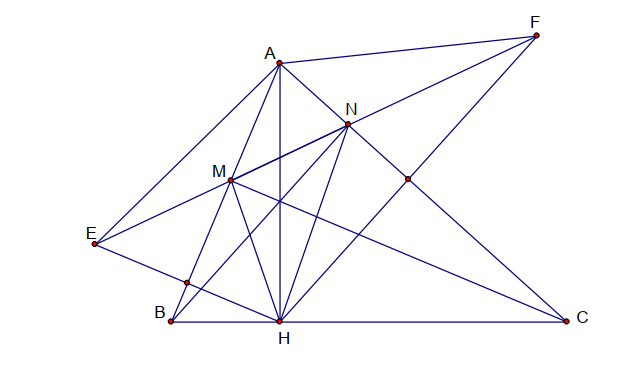
\includegraphics[width=0.7\textwidth]{1-4-lg.png}
    \begin{enumerate}
        \item Vì $\mathrm{AB}$ là trung trực của $\mathrm{EH}$ nên ta có: $\mathrm{AE}=\mathrm{AH}$ (1) \\[10pt]
        Vì $\mathrm{AC}$ là trung trực của $\mathrm{HF}$ nên ta có: $\mathrm{AH}=\mathrm{AF}$ (2) \\[10pt]
        Từ (1) và $(2)$ suy ra: $\mathrm{AE}=\mathrm{AF}$
        \item Vì $\mathrm{M} \in \mathrm{AB}$ nên $\mathrm{MB}$ là phân giác $E M H \Rightarrow \mathrm{MB}$ là phân giác ngoài góc $\mathrm{M}$ của tam giác $\mathrm{MNH}$ \\[10pt]
        Vì $\mathrm{~N} \in \mathrm{AC}$ nên $\mathrm{NC}$ là phân giác $F N H \Rightarrow \mathrm{NC}$ là phân giác ngoài góc $\mathrm{N}$ của tam giác MNH \\[10pt]
        Do $\mathrm{MB}$; $\mathrm{NC}$ cắt nhau tại $\mathrm{A}$ nên $\mathrm{HA}$ là phân giác trong góc $\mathrm{H}$ của tam giác $\mathrm{HMN}$ hay HA là phân giác của $M H N$.
        \item Ta có $\mathrm{AH} \perp \mathrm{BC}$ (gt) mà $\mathrm{HM}$ là phân giác $M H N \Rightarrow \mathrm{HB}$ là phân giác ngoài góc $\mathrm{H}$ của tam giác $\mathrm{HMN}$ \\[10pt]
        $M B$ là phân giác ngoài góc $M$ của tam giác $\mathrm{HMN}(\mathrm{cmt}) \Rightarrow \mathrm{NB}$ là phân giác trong góc $\mathrm{N}$ của tam giác $\mathrm{HMN}$ \\[10pt]
        $\Rightarrow \mathrm{BN} \perp \mathrm{AC}$ ( Hai đường phân giác của hai góc kề bù thì vuông góc với nhau). $\Rightarrow$ $\mathrm{BN} / / \mathrm{HF}$ ( cùng vuông góc với $\mathrm{AC}$ )
        Chứng minh tương tự ta có: $\mathrm{EH} / / \mathrm{CM}$
    \end{enumerate}
}
\end{bt}
	\section{Đề số 2}

\begin{bt} 
    \begin{enumerate}[a.]
        \item Thực hiện phép tính: $\mathrm{A}=\frac{2^{12} \cdot 3^5-4^6 \cdot 9^2}{2^2 \cdot 3^6+8^4 \cdot 3^5}-\frac{5^{10} .7^3-25^5 .49^2}{125.7^3+5^9 \cdot 14^3}$
        \item Tính giá trị biểu thức: $\quad B=1.2 .3+2.3 .4+3.4 .5+4.5 .6+\ldots+17.18 .19$
        \item Tìm một số tự nhiên có 3 chữ số, biết rằng nếu tăng chữ số hàng trăm thêm $\mathrm{n}$ đơn vị đồng thời giảm chữ số hàng chục và giảm chữ số hàng đơn vị đi n đơn vị thì được một số có 3 chữ số gấp n lần số có 3 chữ số ban đầu.
    \end{enumerate}
\loigiai{} 
\end{bt}

\begin{bt}
    \begin{enumerate}[a.]
        \item Tìm các số $x, y, z$ biết rằng: $\quad 3 x=4 y, 5 y=6 z$ và $x y z=30$.
        \item Tìm $x$ biết:
    $$
    \left|\mathrm{x}-\frac{1}{2}\right|+\frac{3}{4}=\left|-1,6+\frac{3}{5}\right|
    $$
    \end{enumerate}
\loigiai{} 
\end{bt}

\begin{bt}
    \begin{enumerate}[1.]
        \item Cho hàm số $\mathrm{y}=\mathrm{f}(\mathrm{x})=(\mathrm{m}-1) \mathrm{x}$
           \begin{enumerate}[a.]
            \item Tìm m biết: $f(2)-f(-1)=7$.
            \item Cho $m=5$. Tìm $x$ biết $f(3-2 x)=20$
           \end{enumerate}
        \item Cho các đơn thức $\mathrm{A}=-\frac{1}{2} \mathrm{x}^2 \mathrm{yz}^2, \mathrm{~B}=-\frac{3}{4} \mathrm{xy}^2 \mathrm{z}^2, \mathrm{C}=\mathrm{x}^3 \mathrm{y}$\\
        Chứng minh rằng các đơn thức $\mathrm{A}, \mathrm{B}, \mathrm{C}$ không thể cùng nhận giá trị âm.
    \end{enumerate}
\loigiai{} 
\end{bt}

\begin{bt}
    Cho $\triangle \mathrm{ABC}$ nhọn có góc $\mathrm{A}$ bằng $60^{\circ}$. Phân giác $\mathrm{ABC}$ cắt $\mathrm{AC}$ tại $\mathrm{D}$, phân giác $\mathrm{ACB}$ cắt $A B$ tại E. BD cắt $C E$ tại I.
    \begin{enumerate}[a.]
    \item Tính số đo góc BIC.
    \item Trên cạnh $\mathrm{BC}$ lấy điểm $\mathrm{F}$ sao cho $\mathrm{BF}=\mathrm{BE}$. Chứng minh $\Delta \mathrm{CID}=\Delta \mathrm{CIF}$.
    \item Trên tia IF lấy điểm $\mathrm{M}$ sao cho $\mathrm{IM}=\mathrm{IB}+\mathrm{IC}$. Chứng minh $\triangle \mathrm{BCM}$ là tam giác đều.
    \end{enumerate}
\loigiai{}
\end{bt}

\begin{bt}
    Tìm số tự nhiên $\mathrm{n}$ thỏa mãn điều kiện: $\quad 2 \cdot 2^2+3 \cdot 2^3+4 \cdot 2^4+\ldots+\mathrm{n} \cdot 2^{\mathrm{n}}=2^{\mathrm{n}+11}$
\loigiai{}
\end{bt}
	\onehalfspacing
\section{Đề số 3}
\graphicspath{{./img/}}
\begin{bt} 
    Cho $\mathrm{x}, \mathrm{y}, \mathrm{z}$ là các số khác 0 và $\mathrm{x}^2=\mathrm{yz}, \mathrm{y}^2=\mathrm{xz}, \mathrm{z}^2=\mathrm{xy}$.\linebreak[2]
    Chứng minh rằng: $\mathrm{x}=\mathrm{y}=\mathrm{z}$.
\loigiai{
    Vì $\mathrm{x}, \mathrm{y}$, $\mathrm{z}$ là các số khác 0 và $\mathrm{x}^2=\mathrm{yz}, \mathrm{y}^2=\mathrm{xz}, \mathrm{z}^2=\mathrm{xy}$ \\[5px]
     $\Rightarrow \frac{x}{y}=\frac{z}{x} ; \frac{y}{z}=\frac{x}{y} ; \frac{z}{x}=\frac{y}{z}$\\[5px] 
     $\Rightarrow \frac{x}{y}=\frac{y}{z}=\frac{z}{x}$\\[5px] 
     Áp dụng tính chất dãy tỉ số bằng nhau $\Rightarrow \frac{x}{y}=\frac{y}{z}=\frac{z}{x}=\frac{x+y+z}{y+z+x}=1 \Rightarrow x=y=z$
} 
\end{bt}

\begin{bt}
    \hfill
    \begin{enumerate}[a.]
        \item Tìm $x$ biết: $5^x+5^{x+2}=650$
        \item Tìm số hữu tỷ $x, y$ biết: $(3 x-33)^{2008}+|y-7|^{2009} \leq 0$
    $$
    \left|\mathrm{x}-\frac{1}{2}\right|+\frac{3}{4}=\left|-1,6+\frac{3}{5}\right|
    $$
    \end{enumerate}
\loigiai{
    \begin{enumerate}
        \item $
            5^x+5^{x+2}=650 \\[5px]
            \Leftrightarrow 5^x\left(1+5^2\right)=650 \\[5px]
            \Leftrightarrow 5^x .26=650 \\[5px]
            \Leftrightarrow \quad 5^x=25 \\[5px]
            \Leftrightarrow \quad 5^x=5^2 \\[5px]
            \Rightarrow x=2
            $
        \item $
            \text {Ta có }(3 \mathrm{x}-33)^{2008} \geq 0 \\[5px]
            |y-7|^{2009} \geq 0 \\[5px]
            \text { Suy ra }(3 \mathrm{x}-33)^{2008}+|y-7|^{2009} \geq 0 \\[5px]
            \text { Mà } \quad(3 \mathrm{x}-33)^{2008}+|y-7|^{2009} \leq 0 \text { (Theo đề bài ) } \\[5px]
            \text { Nên }(3 \mathrm{x}-33)^{2008}+|y-7|^{2009}=0 \\[5px]
            \Leftrightarrow(3 \mathrm{x}-33)^{2008}=0 \text { và }|y-7|^{2009}=0 \\[5px]
            \Leftrightarrow \mathrm{x}=11 \text { và } \mathrm{y}=7
            $
    \end{enumerate}
} 
\end{bt}

\begin{bt}
    Cho hàm số : $\mathrm{f}(\mathrm{x})=\mathrm{a} .\mathrm{x}^2+\mathrm{b} . \mathrm{x}+\mathrm{c}$ với $\mathrm{a}, \mathrm{b}, \mathrm{c}, \mathrm{d} \in \mathrm{Z}$

    Biết $f(1) \vdots 3 ; f(0) \vdots 3 ; f(-1) \vdots 3$. Chứng minh rằng $\mathrm{a}, \mathrm{b}, \mathrm{c}$ đều chia hết cho 3
\loigiai{
    Ta có: $\mathrm{f}(0)=\mathrm{c} ; \mathrm{f}(1)=\mathrm{a}+\mathrm{b}+\mathrm{c} ; \mathrm{f}(-1)=\mathrm{a}-\mathrm{b}+\mathrm{c}$
$$
\begin{aligned}
& \text { +) } f(0) \vdots 3 \Rightarrow c \vdots 3 \\[5px]
& \text { +) } f(1) \vdots 3 \Rightarrow a+b+c \vdots 3 \Rightarrow a+b \vdots 3(1) \\[5px]
& \text { +) } f(-1) \vdots 3 \Rightarrow a-b+c \vdots 3 \Rightarrow a-b \vdots 3(2)
\end{aligned}
$$
Từ (1) và (2) Suy ra $(\mathrm{a}+\mathrm{b})+(\mathrm{a}-\mathrm{b}) \vdots 3 \Rightarrow 2 a \vdots 3 \Rightarrow a \vdots 3$ vì $(2 ; 3)=1 \Rightarrow b \vdots 3$\\[5px]
Vậy a , b , c đều chia hết cho 3
} 
\end{bt}

\begin{bt}
    Cho tam giác $\mathrm{ABC}, \mathrm{AD}$ là tia phân giác của góc $\mathrm{A}$ và $B>C$.
    \begin{enumerate}[a.]
    \item Chứng minh rằng $A D C-A D B=B-C$.
    \item Vẽ đường thẳng $\mathrm{AH}$ vuông góc $\mathrm{BC}$ tại $\mathrm{H}$. Tính $A D B$ và $H A D$ khi biết $B-C=40^{\circ}$
    \item Vẽ đường thẳng chứa tia phân giác ngoài của góc đỉnh $\mathrm{A}$, nó cắt đường thẳng $\mathrm{BC}$
    tại E. 
    
    Chứng minh rằng $A E B=H A D=\frac{B-C}{2}$
    \end{enumerate}
\loigiai{
    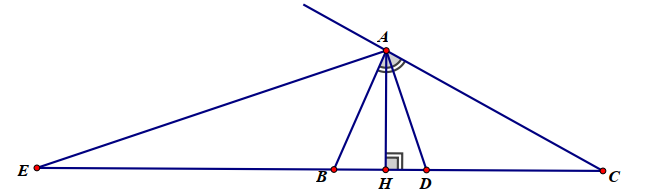
\includegraphics[width=0.7\textwidth]{3-4-lg.png}
    \begin{enumerate}
        \item $A D C=B+B A D \quad($ góc ngoài $\triangle \mathrm{ABD})(1)$\\[5px]
        $A D B=C+C A D$ ( góc ngoài $\triangle \mathrm{ADC})(2)$
        Mà $\mathrm{AD}$ là phân giác góc $\mathrm{BAD}$ nên $B A D=D A C(3)$\\[5px]
        Từ $(1),(2)$ và (3) suy ra đpcm
        \item
        Ta có:
        $$
        \begin{aligned}
        & A D C-A D B=B-C=40^{\circ} \\[5px]
        & A D C+A D B=180^{\circ} \\[5px]
        & \Rightarrow A D C=\frac{180^{\circ}+40^{\circ}}{2}=110^{\circ} ; A D B=70^{\circ} \\[5px]
        & \Rightarrow A H D=20^{\circ}
        \end{aligned}
        $$
        \item
        Ta có $\mathrm{AD}, \mathrm{AE}$ là hai tia phân giác của hai góc kê bù đỉnh $\mathrm{A}$ nên $\mathrm{AD} \perp \mathrm{AE}$\\[5px]
        Xét $\triangle \mathrm{AED} \quad$ ta có: $A E B+A D E=90^{\circ}$ (4)\\[5px]
        Xét $\triangle \mathrm{AHD}$ ta có: $H A D+A D E=90^{\circ}$ (5)\\[5px]
        Mặt khác\\[5px]
        $A D B=C+D A C=C+\frac{A}{2}$ \\[5px]
        $A+B+C=180^{\circ}$ \\[5px]
        $\Rightarrow \frac{A}{2}=90^{\circ}-\frac{B+C}{2}$ \\[5px]
        $A D B=C+90^{\circ}-\frac{B+C}{2}$ \\[5px]
        $\quad=\frac{C-B}{2}+90^{\circ}$ \\[5px]
        $\frac{\mathrm{B}-C}{2}+A D B=90^{\circ}(6)$\\[5px]
        Từ (4), (5) và (6) suy ra đpcm
    \end{enumerate}
}
\end{bt}

\begin{bt}
    \hfill
    \begin{enumerate}[a.]
        \item  Cho $S=1-\frac{1}{2}+\frac{1}{3}-\frac{1}{4}+\ldots+\frac{1}{2011}-\frac{1}{2012}+\frac{1}{2013}$ và $P=\frac{1}{1007}+\frac{1}{1008}+\ldots+\frac{1}{2012}+\frac{1}{2013}$.
        
        Tính $(S-P)^{2013}$.
        \item Cho $\mathrm{A}=\frac{\sqrt{x}+1}{\sqrt{x}-3}$
        
        Tìm $\mathrm{x} \in \mathrm{Z}$ để $\mathrm{A}$ có giá trị là một số nguyên.
    \end{enumerate}
\loigiai{
    \begin{enumerate}
        \item Ta có: \\[5px]
        $$
\begin{aligned}
& P=\frac{1}{1007}+\frac{1}{1008}+\ldots+\frac{1}{2012}+\frac{1}{2013} \\[5px]
& =\left(1+\frac{1}{2}+\frac{1}{3}+\ldots+\frac{1}{1006}+\frac{1}{1007}+\frac{1}{1008}+\ldots+\frac{1}{2012}+\frac{1}{2013}\right)-\left(1+\frac{1}{2}+\frac{1}{3}+\ldots+\frac{1}{1006}\right) \\[5px]
& =\left(1+\frac{1}{2}+\frac{1}{3}+\ldots+\frac{1}{1006}+\frac{1}{1007}+\frac{1}{1008}+\ldots+\frac{1}{2012}+\frac{1}{2013}\right)-2\left(\frac{1}{2}+\frac{1}{4}+\frac{1}{6}+\ldots+\frac{1}{2012}\right) \\[5px]
& =1-\frac{1}{2}+\frac{1}{3}-\frac{1}{4}+\ldots \ldots-\frac{1}{2012}+\frac{1}{2013}=S .
\end{aligned}
$$
Do đó $(S-P)^{2013}=0$
\item
Tìm $x \in z$ đề $A \in Z$
$$
\mathrm{A}=\frac{\sqrt{x}+1}{\sqrt{x}-3}=1+\frac{4}{\sqrt{x}-3} \quad(\mathrm{dk} \quad \mathrm{x} \geq 0, \mathrm{x} \neq 9)
$$
A nguyên khi $\frac{4}{\sqrt{x}-3}$ nguyên $\Rightarrow \sqrt{x}-3$ là Ư (4)
$$
\text{Ư}(4)=\{-4 ;-2 ;-1 ; 1 ; 2 ; 4\}
$$
Các giá trị của $x$ là : $1 ; 4 ; 16 ; 25 ; 49$.
    \end{enumerate}
}
\end{bt}
	\section{Đề số 4}

\begin{bt} 
   \hfill
   \begin{enumerate}[a.]
    \item Thực hiện phép tính: $\mathrm{A}=\left[\left(\frac{2}{193}-\frac{3}{386}\right) \cdot \frac{193}{17}+\frac{33}{34}\right]:\left[\left(\frac{7}{1931}+\frac{11}{3862}\right) \cdot \frac{1931}{25}+\frac{9}{2}\right]$.
    \item Rút gọn :    
    $$
    \mathrm{B}=(-5)^0+(-5)^1+(-5)^2+(-5)^3+\ldots+(-5)^{2016}+(-5)^{2017}
    $$
   \end{enumerate}
\loigiai{} 
\end{bt}

\begin{bt}
    \hfill
    \begin{enumerate}[a.]
        \item Tìm a, b, c biết $\quad \frac{12 a-15 b}{7}=\frac{20 c-12 a}{9}=\frac{15 b-20 c}{11}$ và $a+b+c=48$.
        \item Một công trường dự định phân chia số đất cho ba đội I, II, III tỉ lệ với 7; 6; 5 . Nhưng sau đó vì số người của các đội thay đổi nên đã chia lại tỉ lệ với $6 ; 5 ; 4$. Như vậy có một đội làm nhiều hơn so với dự định là $6 \mathrm{m}^3$ đất. Tính tổng số đất đã phân chia cho các đội.
    \end{enumerate}
\loigiai{} 
\end{bt}

\begin{bt}
   \hfill
   \begin{enumerate}[a.]
    \item Tìm giá trị nhỏ nhất của biểu thức: $C=\frac{|x-2017|+2018}{|x-2017|+2019}$.
    \item Chứng tỏ rằng $\mathrm{S}=\frac{3}{4}+\frac{8}{9}+\frac{15}{16}+\ldots+\frac{\mathrm{n}^2-1}{\mathrm{n}^2}$ không là số tự nhiên với mọi $\mathrm{n} \in \mathrm{N}, \mathrm{n}>$2.
    \item Tìm tất cả các cặp số nguyên $x$, $y$ sao cho: $x-2 x y+y=0$.
   \end{enumerate}
\loigiai{} 
\end{bt}

\begin{bt}
    Cho tam giác cân $A B C, A B=A C$. Trên cạnh $B C$ lấy điểm $D$, trên tia đối của $C B$ lấy điểm $\mathrm{E}$ sao cho $\mathrm{BD}=\mathrm{CE}$. Các đường thẳng vuông góc với $\mathrm{BC}$ kẻ từ $\mathrm{D}$ và $\mathrm{E}$ cắt $\mathrm{AB}$ và $A C$ lân lượt ở $M$ và $N$. Chứng minh rằng: 
    \begin{enumerate}[a.]
    \item $\mathrm{DM}=\mathrm{EN}$.
    \item Đường thẳng $\mathrm{BC}$ cắt $\mathrm{MN}$ tại điểm $\mathrm{I}$ là trung điểm của $\mathrm{MN}$.
    \item Đường thẳng vuông góc với $\mathrm{MN}$ tại I luôn luôn đi qua một điểm cố định khi $\mathrm{D}$ thay đổi trên cạnh BC.
    \end{enumerate}
\loigiai{}
\end{bt}

\begin{bt}
    \hfill
    Trong hình bên, đường thẳng $\mathrm{OA}$ là đồ thị của hàm số $\mathrm{y}=\mathrm{f}(\mathrm{x})=\mathrm{ax}$.
    \begin{enumerate}[a.]
        \item  Tính tỉ số $\frac{\mathrm{y}_0-2}{\mathrm{x}_0-4}$.
        \item Giả sử $x_0=5$. Tính diện tích tam giác $\mathrm{OBC}$
    \end{enumerate}
\loigiai{}
\end{bt}
\end{document}